\documentclass[]{book}
\usepackage[portuguese]{babel}
\usepackage[utf8]{inputenc}
\usepackage{graphicx}
\usepackage{hyperref}
\usepackage{mdwlist}
%\usepackage{pslatex}
\usepackage{charter}
\usepackage[margin=2cm]{geometry}
\usepackage{makeidx}

% Title Page
\title{\textbf{Introdução à simulação de circuitos com o \textit{LTspice}}}
\author{Renan Birck Pinheiro}

\begin{document}

\begin{titlepage}
\begin{center}

\textsc{\LARGE Universidade Federal de Santa Maria}\\[1.5cm]
\textsc{\Large Centro de Tecnologia}\\[0.5cm]
\textsc{\Large II Jornada de Minicursos}\\[0.5cm]

\end{center}

\vspace*{5cm}
\begin{center}
{\huge \bfseries Introdução à Simulação de Circuitos com o \textit{LTspice}}\\[0.4cm]
\vspace*{130px}
\emph{Autor:}
Renan Birck Pinheiro <\url{renan.ee.ufsm@gmail.com}>


Santa Maria, \today.

\end{center}




\end{titlepage}

\tableofcontents

\chapter{Introdução}
As primeiras versões do SPICE (\textit{Simulation Program with Integrated Circuit Emphasis}\footnote{Programa de Simulação com Ênfase em Circuitos Integrados}) foram desenvolvidas nos anos 70, visando (como o próprio nome já diz) a simulação de circuitos integrados (atividade na qual é inviável ou impossível a prototipagem). Inicialmente, devido aos limitados recursos computacionais da época, as simulações eram restritas a circuitos simples, e os resultados - após a simulação ser executada em computadores de grande porte - eram visualizados de forma textual.

Na década de 80, o SPICE foi portado do FORTRAN para o C e passou a ser executado no ambiente UNIX (versão chamada de SPICE3), permitindo o uso em computadores de pequeno/médio porte e \textit{workstations} com interfaces gráficas simples. 

Já nos anos 90, com o aumento exponencial da capacidade dos computadores pessoais, desenvolveram-se versões deste - com interfaces gráficas sofisticadas - para os sistemas operacionais mais utilizados, assim possibilitando o uso da ferramenta sem necessidade de contato com a linha de comando. Apesar destas mudanças, o mecanismo de funcionamento de um simulador  efetivamente permanece o mesmo: empregam-se as equações e análises da teoria dos circuitos, junto com métodos numéricos e modelos equivalentes para semicondutores e outros dispositivos, para a análise numérica do circuito. Não iremos entrar nos detalhes sobre esses algoritmos: os interessados podem ex. verificar \cite{nagel} e \cite{chung}.

No presente trabalho serão abordados os conceitos básicos do uso do software, suficientes para os usos mais comuns a serem encontrados durante a graduação. Assuntos mais avançados, que infelizmente não podem ser abordados por questão de tempo, estão disponíveis no sistema de ajuda (aperte F1 dentro do \textit{LTspice}).
\chapter{A interface do \textit{LTspice}}
O LTspice pode ser baixado a partir do site da \textit{Linear Technology}: \url{http://www.linear.com/ltspice}, selecionando-se a opção \textit{Download LTspice IV} e, após, a opção \textit{No, thanks, just download the software}. 

Após instalado, o \textit{LTspice} pode ser aberto a partir do Menu Iniciar ou do ícone criado na área de trabalho. Então, teremos a interface dele:

\begin{figure}[htb]
\center 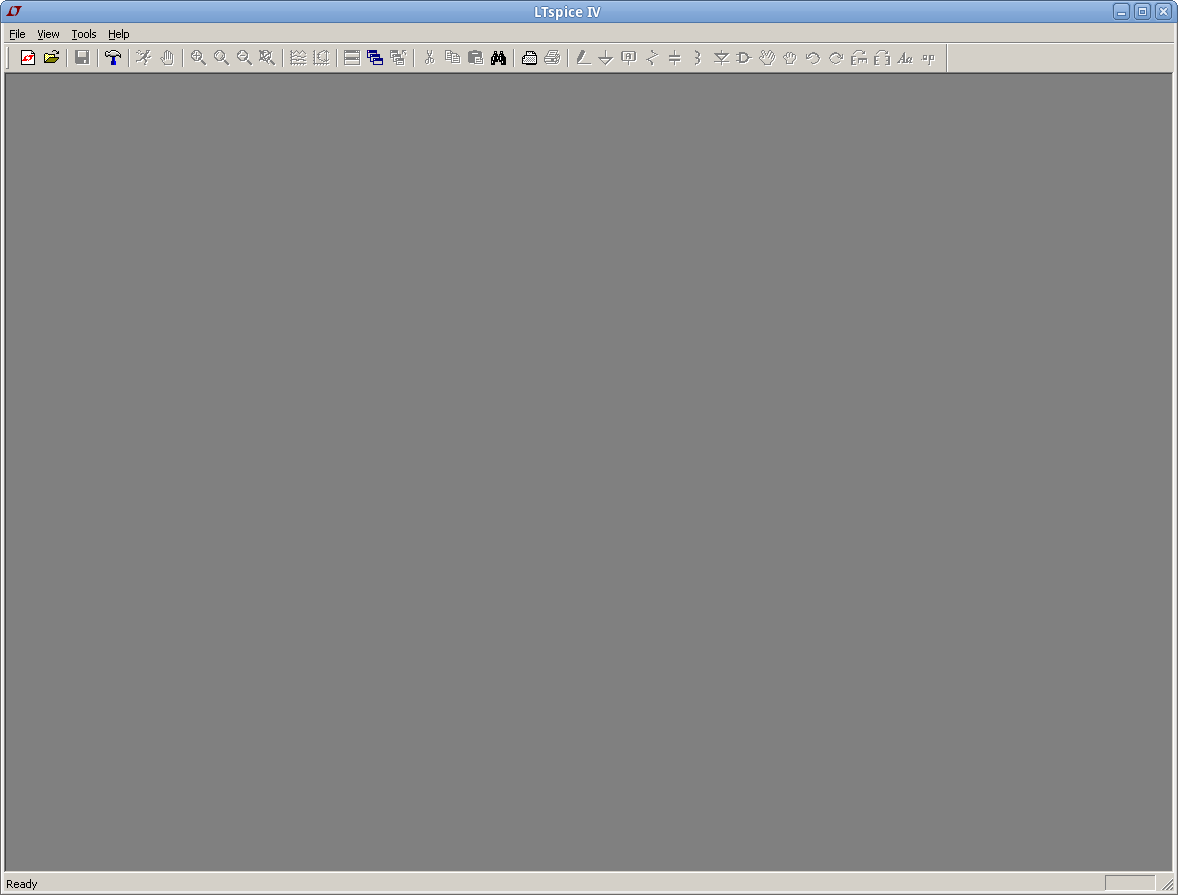
\includegraphics[width=400px]{imagens/ltspice_janela_principal}
\caption{A tela principal do LTspice. Clique no botão \textit{New Schematic} para criar um novo desenho, ou no botão \textit{Open} para abrir um esquemático existente.}
\end{figure}

\chapter{Links úteis e contato}
\begin{itemize}
\item \url{http://tech.groups.yahoo.com/group/LTspice/} - grupo de usuários do LTspice
\end{itemize}

O autor pode ser contatado atráves de:

\begin{itemize}
\item e-mail/Google Talk: \url{renan.ee.ufsm@gmail.com}
\item Facebook: \url{http://facebook.com/renanbirck}
\item Twitter: \url{http://twitter.com/birckrenan}
\item Fork me on GitHub: \url{http://github.com/renanbirck}
\end{itemize}

\bibliographystyle{abbrv}
\bibliography{apostila_LTspice}

\end{document}          
